\documentclass[a4paper, 12pt]{report}

\author{Deniz Güven}

\usepackage[ngerman]{babel}
\usepackage[utf8]{inputenc}
\usepackage[T1]{fontenc}
\usepackage{minted}
\usepackage{tikz}
\usetikzlibrary{arrows, automata}
\usepackage{xcolor}
\usepackage{forest}
\usepackage{graphicx}
\usepackage{fancyhdr}
\usepackage{amsmath, amsfonts, amssymb, amsthm}
\usepackage{mathtools}
\usepackage{stmaryrd}
\usepackage[parfill]{parskip}
\usepackage[colorlinks]{hyperref}
\usepackage[]{cleveref} % to be loaded after hyperref
\usepackage{verbatim}
\usepackage[shortcuts]{extdash}
\usepackage[margin=2cm]{geometry}

\crefname{equation}{}{}

\begin{document}

%TITLE PAGE
\begin{titlepage}
  \begin{center}
    
\includegraphics[width=0.5\linewidth]{res/uni.png}
    \vspace{2cm}

    \huge{\textbf{Berechnung von Molekül-Grundzustandsenergien 
    mit Ab-Initio-Methoden}}
    \vspace{1cm}

    \Large
    Fachbereich Informatik

    Bachelorarbeit

    Deniz Güven
    \vfill

    Betreuer: 

    \today
  \end{center}
\end{titlepage}

\tableofcontents


%INTRODUCTION
\chapter{Einleitung}
\section{Hintergrund}
Die Chemie im Allgemeinen befasst sich mit den Eigenschaften und Interaktionen
von Molekülen bzw. Atomen. Es ist also von hohem Interesse diese
durch akkurate Modelle zu beschreiben. In der Chemie, wie mit allen
Naturwissenschaften, wurden im Laufe der Geschichte immer genauere Theorien entwickelt.
Im 20. Jahrhundert kam es dann zur Begründung der Computerchemie durch die Einführung zweier 
revolutionärer Gebiete, die der Quantenphysik und der Informatik.
Nun war es nicht nur möglich chemische Systeme auf vorher ungesehene Genauigkeit zu beschreiben,
sondern auch noch quantitative Berechnungen mit Computern an diesen durchzuführen.
Deshalb handelt es sich bei der Computerchemie möglicherweise zukünftig
um eines der nützlichesten Werkzeuge in der Chemie.

\begin{figure}[h]
    \begin{center}
    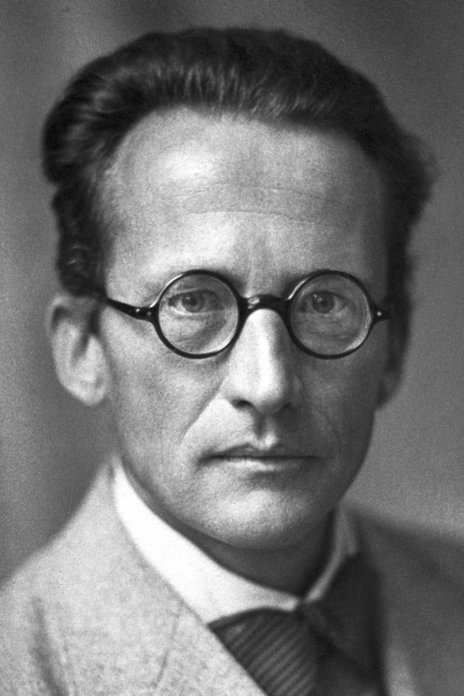
\includegraphics[width=0.25\textwidth]{res/schrodinger.jpg}
    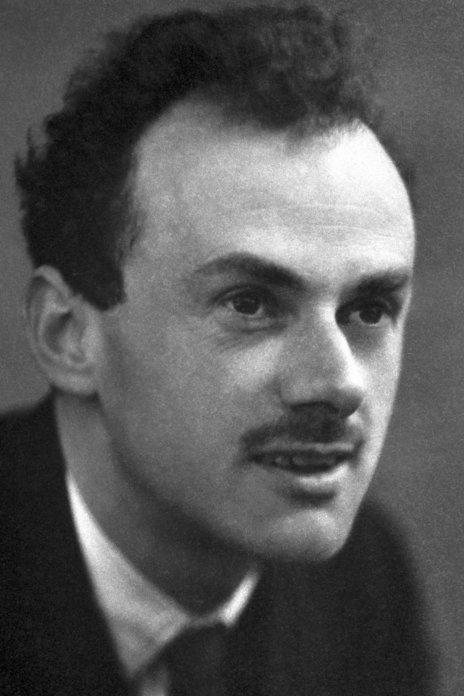
\includegraphics[width=0.25\textwidth]{res/dirac.jpg}
\end{center}
    \caption{Erwin Schrödinger und Paul Adrien Maurice Dirac wurden 1933 mit dem Nobelpreis
    für Physik ausgezeichnet für ihre Entdeckungen im Bezug auf die Atomtheorie. \cite{nobel_1933}}
\end{figure}

\section{Ziele}
Wegen der hohen Komplexität und Weitläufigkeit der Computerchemie
kann der Einstieg oft schwierig sein. Aus diesem Grund wird
in dieser Arbeit versucht eine Übersicht der notwendigen Theorie zu geben,
um selber einfache quantenchemische Berechnungen durchzuführen.
Zudem wird noch eine eigene Implementierung
zur Theorie bereitgestellt und besprochen.

Zum Einstieg bietet sich die Berechnung von einem grundlegenden Wert
innerhalb der Hartree-Fock-Theorie an, die Hartree\-/Fock\-/Energie, 
mit dieser können viele Prozesse in der Chemie,
wie Reaktionsabläufe und Molekülstrukturen, erklärt werden.
Um diese Energie zu berechnen, wird im Folgenden
die Hartree\-/Fock\-/Theorie entwickelt und angewendet.


\section{Einordnung der Hartee\-/Fock\-/Theorie in der Chemie} \label{posthf}
Die HF\-/Theorie gehört zur Klasse der Ab\-/Initio\-/Methoden,
welche versuchen nur basierend auf theoretischen Modellen und
universellen Konstanten Berechnung durchzuführen.
\cite[5.1, 5.2.2]{lewars_2016}

Diese Verfahren stehen im Gegensatz zu den Semiempirischen\-/Methoden,
welche zusätzliche experimentell bestimmte Werte in die Berechnungen einbinden.
\cite[S. 421]{lewars_2016}

Die HF-Theorie ist der einfachste noch praktisch verwendete Vertreter
der Klasse der Ab\-/Initio\-/Methoden
und wird deshalb bei entweder sonst zu großen System oder
als Start-Approximation für sehr akkurate Berechnungen verwendet.
\cite[S. 433]{structure_2013}

Basierend auf der HF-Theorie existieren die Post\-/Hartree\-/Fock\-/Methoden,
diese verbesseren die Genauigkeit der Ergebnisse hauptsächlich
durch eine genauere Behandlung der Elektron-Elektron-Interaktionen.
\cite[5.4]{lewars_2016}

Neben den Post\-/HF\-/Methoden existieren zudem Verfahren
mit unterschiedlichen Ansätzen. Eine der relevantesten ist
die Dichte\-/Funktional\-/Theorie (DFT), welche nicht auf
Wellenfunktionen aufbaut sondern direkt mit den
Dichtefunktionen der Elektronen arbeitet.
\cite[7.1]{lewars_2016}

%THEORY
\chapter{Theorie und Methoden}

\section{Allgemeine Theorie}

\subsection{Grundlegende Definitionen und Notation}
Um Moleküle in einem quantenmechanischen Modell zu beschreiben,
müssen wir zunächst einige Definitionen aufstellen:

\subsubsection{Wellenfunktionen}

Die sogenannte Wellenfunktion $\Psi(x_1, x_2, \dots)$ 
beschreibt den Zustand eines quantenmechanischen Systems vollständig.
Im Kontext eines Moleküls entspricht dies der Wellenfunktion für die Atomkerne
und deren Elektronen.

Zu den Wellenfunktionen $\psi, \varphi$ wird ein Skalarprodukt definiert:
\begin{equation}
    \langle \psi(x) \vert \varphi(x) \rangle \equiv  \int \psi^*(x) \phi(x) \,dx
\end{equation}
Das Integral geht über den gesamten Raum aller Parameter.

Das Betragsquadrat der Wellenfunktion $\vert \Psi \vert^2$
lässt sich dabei als Wahrscheinlichkeitsdichte interpretieren, wenn $\Psi$ normiert ist
($\langle \Psi \vert \Psi \rangle = 1$).

\cite[S. 20-21, 24]{atkins_friedman_2011}

In der restlichen Arbeit gehen wir immer von normierten Wellenfunktionen aus.
Sollten die Parameter nicht von direkter Relevanz sein, werden diese weggelassen.

\subsubsection{Operatoren}
Beobachtbare Eigenschaften eines quantenmechanischen Systems 
werden durch sogenannte Operatoren repräsentiert.
Diese Operatoren werden über das Hut\-/Symbol (zb.: $\hat{o}$) gekennzeichnet
und müssen hermitesch sein.
Ein Operator $\hat{o}$ wirkt auf ein quantenmechanisches System $\varphi$
und verändert diesen in einen anderen Zustand $\psi$.

Wir binden hermitesche Operatoren $\hat{o}$ noch in unsere Notation für das Skalarprodukt ein,
sodass sich schreiben lässt:
\begin{equation}
    \langle \psi(x) \vert \hat{o} \vert \varphi(x) \rangle \equiv
    \int \psi^*(x) \hat{o} \varphi(x) \,dx
\end{equation}

Ist das System $\varphi$ eine Eigenfunktion des Operators $\hat{o}$,
erhalten wir eine Eigenwertsgleichung mit dem Eigenwert $\lambda$:
\begin{equation}
    \hat{o} \varphi = \lambda \varphi
\end{equation}
Außerdem gilt für das Skalarprodukt mit sich selbst dann:
\begin{equation}
    \langle \varphi(x) \vert \hat{o} \vert \varphi(x) \rangle = \lambda
\end{equation}

Sollte $\varphi$ keine Eigenfunktion eines Operators $\hat{o}$ sein,
so kann man den Erwartungswert der Eigenschaft, welche durch $\hat{o}$ ausgedrückt wird, bestimmen über:
\begin{equation}
\langle \psi(x) \vert \hat{o} \vert \psi(x) \rangle
  = \int \psi^*(x) \hat{o} \psi(x) \,dx
\end{equation}

\cite{tc1_ops}
\cite[S. 21]{atkins_friedman_2011}
\cite[S. 155-156]{levine_2019}

\subsubsection{Die Schrödingergleichung}
Im Rahmen dieser Arbeit gehen wir von nur zeitlich statischen Systemen aus,
welche durch die zeitunabhängige Schrödingergleichung beschrieben werden:
\begin{equation}\label{schroedinger}
  \hat{H}\psi = E\psi
\end{equation}

Durch das Lösen dieser Eigenwerts\-/Gleichung sind wir in der Lage
die Energien und weitere Eigenschaften von Molekülen zu bestimmen.
Der Operator $\hat{H}$ ist der sogenannte Hamiltonian und
gibt die Energie $E$ des Systems wieder.

\cite[S. 24-25]{atkins_friedman_2011}

\subsection{Hamilton-Operator}
Der allgemeine Hamilton\-/Operator für Moleküle mit $N$ Elektronen und $M$ Atomkernen lautet:
\begin{flalign}\label{hamilton}
  \hat{H} &= -\sum_i^N \frac{1}{2} \nabla_i^2 
            -\sum_A^M \frac{1}{2 m_A} \nabla_A^2
            -\sum_i^N \sum_A^M \frac{Z_A}{r_{iA}}
            +\frac{1}{2}\sum_{i\neq j} \frac{1}{r_{ij}}
            +\frac{1}{2}\sum_{A \neq B } \frac{Z_A Z_B}{r_{AB}}\nonumber\\
          &= \hat{T}_e + \hat{T}_a + \hat{V}_{ea} + \hat{V}_{ee} + \hat{V}_{aa}
\end{flalign}
Dabei steht $Z_A$ für die Ladung des Atomkerns $A$ und 
$r$ für den Abstand zwischen Elektronen und/oder Atomkernen.

\cite[S. 6]{tc2_1}

Die einzelnen Terme haben folgende Bedeutungen:
\begin{enumerate}
    \item $\hat{T}_e$,
    die kinetische Energie aller Elektronen.
    \item $\hat{T}_a$,
    die kinetische Energie aller Atomkerne.
    \item $\hat{V}_{ea}$,
    die potenzielle Energie zwischen allen Elektronen und Atomkernen.
    \item $\hat{V}_{ee}$,
    die potenzielle Energie zwischen allen Elektronen untereinander.
    \item $\hat{V}_{aa}$,
    die potenzielle Energie zwischen allen Atomkernen untereinander.
\end{enumerate}

\subsection{Born-Oppenheimer-Näherung}
Aufgrund des hohen Massenunterschieds zwischen Elektronen und Atomkernen
ist der Einfluss der Elektronen auf die Bewegung der trägeren Atomkerne vernachlässigbar.
Deshalb können bei der Berechnung der Elektronen\-/Wellenfunktion 
die Atomkerne approximativ als statisch betrachtet werden.

Dafür wird der allgemeine Hamilton-Operator \cref{hamilton} aufgeteilt:
\begin{flalign}
  \hat{H} &= \hat{T}_e + \hat{T}_a + \hat{V}_{ea} + \hat{V}_{ee} + \hat{V}_{aa} \nonumber\\
          &= \hat{T}_a + \hat{V}_{aa} + \hat{H}_{\text{el}} \nonumber\\
  \hat{H}_{\text{el}} &= \hat{T}_e + \hat{V}_{ea} + \hat{V}_{ee}
\end{flalign}
Wir lösen nun die Schrödingergleichung \cref*{schroedinger}
mit dem elektronischen Hamilton-Operator $\hat{H}_{\text{el}}$.
Bei der Lösung dieser wird eine feste Kerngeometrie angenommen, 
die wir bei dem Operator $\hat{V}_{eA}$ verwenden werden. 
Mit der resultierenden Elektronen\-/Wellenfunktionen 
lässt sich dann eine Gesamte Wellenfunktion unter Einbezug der Atomkerne konstruieren.

\cite[S. 11-14]{tc2_1}

\subsection{Variationsformulierung}
Da eine analytische Lösung zur Schrödingergleichung nur in speziellen Fällen existiert
\cite[S. 195]{lewars_2016},
wird die exakte Wellenfunktion durch eine Test\-/Wellenfunktion approximiert.
Es lässt sich zeigen, 
dass die Energie dieser Test\-/Wellenfunktion $E_{test}$ 
immer über der tatsächlichen Energie $E_0$ liegt.

\subsubsection*{Beweis}
Voraussetzungen:
\begin{enumerate}
  \item Der Hamiltonian $\hat{H}$ hat die Eigenfunktionen $\psi_i^{}$ mit Eigenwerten $E_i^{}$.
  \item Es existiert eine Eigenfunktion $\psi_0^{}$ mit dem niedrigsten  Eigenwert $E_0^{}$.
  \item Alle Eigenfunktion von $\hat{H}$ sind orthonomal zueinander:\\
  $\langle \psi_i^{} \vert \psi_j^{} \rangle = \delta_{ij}^{},\quad\forall i,j$
  \item Die Test-Wellenfunktion lässt sich als Linearkombination der Eigenfunktionen darstellen:
  $\psi_{test}^{} = \sum_{n}^{} c_n^{} \psi_n^{}$
\end{enumerate}

Die Voraussetzungen (1), (3) und (4) sind anzunehmen, da der Hamiltonian hermitesch ist.
Die 2. Voraussetzung hingegen entspricht unserer physikalischen Realität.

Es ist zu zeigen: $E_{test}^{} \geq E_0^{}$ oder $E_{test}^{} - E_0^{} \geq 0$
\begin{flalign*}
  E_{test} - E_0 
  &= \langle \psi_{test}^{} \vert \hat{H} - E_0^{} \vert \psi_{test}^{} \rangle\\
  &= \int \psi_{test}^* (\hat{H} - E_0^{}) \psi_{test}^{} \,dx \quad &\vert \text{ 4. Voraussetzung}\\
  &= \sum_n \sum_m c_n^\ast c_m^{} \int \psi_{n}^* (\hat{H} - E_0^{}) \psi_{m} \,dx 
  \quad &\vert \text{ 1. Voraussetzung}\\
  &= \sum_n \sum_m c_n^\ast c_m^{} \int \psi_{n}^* (E_m^{} - E_0^{}) \psi_{m} \,dx 
  \quad &\vert \text{ 3. Voraussetzung}\\
  &= \sum_n \left\lvert c_n^{} \right\rvert^2 (E_n^{} - E_0^{}) \int \psi_{n}^* \psi_{n} \,dx 
  \quad &\vert \text{ 3. Voraussetzung}\\
  &= \sum_n \left\lvert c_n^{} \right\rvert^2 (E_n^{} - E_0^{})
  \quad &\vert \text{ 2. Voraussetzung}\\
  &\geq 0 &\qed
\end{flalign*}
\cite[S. 187]{atkins_friedman_2011}

\subsection{Beschreibung von Elektronen}\label{section_slater}
Die Form der Wellenfunktion für Elektronen ist in diesem Modell nicht nur 
durch die Schrödingergleichung \cref{schroedinger} gegeben.
Um ein realitätsnahes Bild von Elektronen zu schaffen,
muss die Wellenfunktionen zusätliche Forderungen erfüllen.
Diese unerfassten Eigenschaften sind das intrinsisches Drehmoment des Elektrons,
auch Spin genannt, und die Antisymmetrie der Wellenfunktion
im Bezug auf den Austausch zweier Elektronen.
Wir stellen diese zusätzlichen Forderungen,
weil diese Eigenschaften experimentell beobachtbar sind.
Anzumerken ist, dass diese Bedingungen an die Wellenfunktion 
in einer relativistischen Behandlung von selbst entstehen
und nicht wie hier künstlich eingebaut werden müssen.

\cite[S. 265, 270]{levine_2019}
\cite[4.5.3]{cramer_2004}

\subsubsection*{Notation}
Da jedes Elektron mindestens 3 Parameter ($x, y, z$) zur Beschreibung benötigt,
kann dies bei größeren Systemen schnell unübersichtlich werden.
Deshalb ist es üblich die Parameter eines Elektrons durch eine natürliche Zahl abzukürzen:

\begin{equation}
    \Psi(1, 2, 3, \dots) \equiv  \Psi(x_1, y_1, z_1, \quad
    x_2, y_2, z_2,\quad x_3, y_3, z_3, \quad\dots)
\end{equation}

Diese verkürzte Notation wird in der restlichen Arbeit verwendet.

\subsubsection*{1. Spin}\label{spin-section}
Jedes Elektron verfügt, neben einer räumlichen Ausdehnung, 
auch über einen intrinsischen Spin. 
Ein Elektron kann lediglich zwei Spin\-/Zustände annehmen.
Diese Zustände werden mit den Spinfunktionen $\alpha$ und
$\beta$ dargestellt und sind gegeben durch:
\begin{equation}\label{spin_function}
  \begin{aligned}
    \alpha(\omega) &:= \delta(\omega - \nicefrac{1}{2})\\
    \beta(\omega) &:= \delta(\omega + \nicefrac{1}{2})
  \end{aligned}
\end{equation}
mit den Eigenschaften:
\begin{equation}\label{spin_product}
  \begin{aligned}
    \langle \alpha \vert \alpha \rangle &= \langle \beta \vert \beta \rangle = 1 \\
    \langle \alpha \vert \beta \rangle &= \langle \beta \vert \alpha \rangle = 0
  \end{aligned}
\end{equation}

Die Spinkoordinate $\omega$ existiert separat von den räumlichen Koordinaten $x,y,z$.
Deshalb hängt die Wellenfunktion $\varphi$ eines einzigen Elektrons
von insgesamt vier Parametern ab
und wird als Produkt einer Raum- und Spin\-/Funktion dargestellt.
Im Kontext eines Moleküls werden die Raumwellenfunktionen auch Orbitale genannt, welche
je zwei Elektronen mit entgegengesetztem Spin enthalten können.
Das Produkt der Raum- und Spin\-/Funktion wird deshalb auch als Spinorbital bezeichnet.

\begin{equation}\label{spin}
  \varphi(1) := \varphi(x_1, y_1, z_1, \omega_1) = \begin{cases}
    \psi(x_1, y_1, z_1) \alpha(\omega_1) = \psi(1) \alpha(1)\\
    \psi(x_1, y_1, z_1) \beta(\omega_1) = \psi(1) \beta(1)\\
  \end{cases}
\end{equation}

Zu beachten ist, dass Elektronen nur für die Werte 
$\omega = \pm \nicefrac{1}{2}$ existieren können ($\lvert \varphi \rvert^2 > 0$) und
der Parametersatz eines Elektrons durch eine natürliche Zahl abgekürzt werden kann.

\cite[S. 45]{szabo_ostlund_1996}

Diese Spin-Eigenschaft wurde erstmals im Stern-Gerlach-Experiment (1921) beobachtet, 
welches in Frankfurt am Main durchgeführt wurde.
\cite{tc1_spin}

\begin{figure}[h]
\begin{center}
    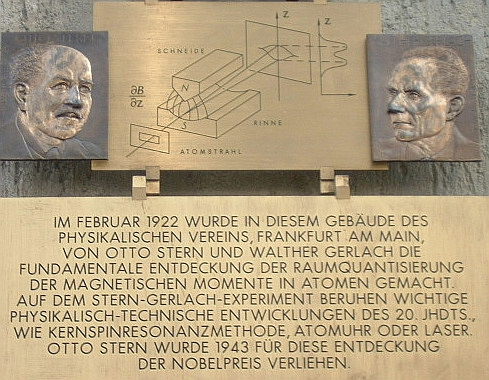
\includegraphics[width=0.75\textwidth]{res/sterngerlach2.jpg}
\end{center}
    \caption{Plakette zum Gedenken an das Stern-Gerlach-Experiment. \cite{sterngerlach}}
\end{figure}


\subsubsection*{2. Antisymmetrie}
Diese Forderung besagt, dass eine Elektronen\-/Wellenfunktion im Bezug auf
den Austausch zweier beliebiger Elektronen\-/Koordinaten antisymmetrisch sein muss:

\begin{equation}\label{antisymmetry}
  \Psi(1, \dots, i, \dots, j, \dots, N) = - \Psi(1, \dots, j, \dots, i, \dots, N), \quad \forall i,j
\end{equation}

\cite[S. 45, 46]{szabo_ostlund_1996}

\subsubsection*{Pauli-Ausschluss-Prinzip}
Aus \cref{spin_product}, \cref{spin} und \cref{antisymmetry} folgt,
dass zwei Elektronen mit identischem Spin sich nicht an
den gleichen Raumkoordinaten aufhalten können. Dies ergibt sich aus folgendem Beweis:

Nehmen wir an, dass zwei Elektronen $i,j$ die selben Raum- und Spin\-/Koordinaten ($i = j$) haben:
\begin{equation*}
  \Psi(1, \dots, i, \dots, j, \dots, N) = \Psi(1, \dots, i, \dots, i, \dots, N)
\end{equation*}
Wir fordern auch Antisymmetrie:
\begin{equation*}
  \Psi(1, \dots, i, \dots, j, \dots, N) = -\Psi(1, \dots, j, \dots, i, \dots, N)
\end{equation*}
Es folgt daher:
\begin{flalign*}
  \Psi(1, \dots, i, \dots, i, \dots, N) &= -\Psi(1, \dots, i, \dots, i, \dots, N) \\
  2\Psi(1, \dots, i, \dots, i, \dots, N) &= 0
\end{flalign*}
$\Rightarrow$ Die Wahrscheinlichkeit, dass zwei Elektronen mit gleichem Spin 
sich am selben Ort befinden ist null. \qed

Dieses Phänomen auf Spinorbitalen angewandt bedeutet,
dass zwei Elektronen nicht das selbe Spinorbital besetzen können,
dies nennt man das Pauli\-/Ausschluss\-/Prinzip.
Das resultierende Meiden der Elektronen wird Pauli\-/Repulsion genannt.

\cite[S. 271, 276]{levine_2019}

\subsubsection*{Slater-Determinante}
Um sowohl Spin als auch die Antisymmetrie in unsere Wellenfunktion einzubinden,
wird diese als Determinante von Spinorbitalen ausgedrückt.
Dabei wird pro Elektron ein Spinorbital verwendet.

\begin{equation}\label{slater}
\Psi(1, \dots, N) = 
\frac{1}{\sqrt{N!}}
\left\lvert
\begin{array}{ccccc} 
\varphi_1(1)  & \varphi_2(1)  & \cdots & \varphi_{N-1}(1)  & \varphi_N(1)\\ 
\varphi_1(2)  & \varphi_2(2)  & \cdots & \varphi_{N-1}(2)  & \varphi_N(2)\\ 
\vdots        & \vdots        & \ddots & \vdots            & \vdots      \\ 
\varphi_1(N)  & \varphi_2(N)  & \cdots & \varphi_{N-1}(N)  & \varphi_N(N)
\end{array}
\right\rvert
\end{equation}

Vertauschen wir zwei Elektronen, gleicht das einem Tausch zweier Zeilen
und das Vorzeichen der Determinante ändert sich.
Die Antisymmetrie unserer Wellenfunktion ist gegeben.

Sollten zwei Elektronen das selbe Spinorbital besetzen,
so wären zwei Spalten identisch, wodurch die Determinante verschwindet.
Das Pauli\-/Ausschluss\-/Prinzip ist ebenfalls erfüllt.

\cite[S. 50]{szabo_ostlund_1996}

Sollte jedes Raumorbital doppelt besetzt sein,
so können wir $\Psi$ mit nur $n$ Raumorbitalen ($2n = N$) darstellen:
\begin{equation}
\Psi(1, \dots, 2n) = 
\frac{1}{\sqrt{(2n)!}}
\left\lvert
\begin{array}{ccccc} 
\psi_1(1)\alpha(1) & \psi_1(1)\beta(1) & \cdots & \psi_n(1)\alpha(1) & \psi_n(1)\beta(1)\\ 
\psi_1(2)\alpha(2) & \psi_1(2)\beta(2) & \cdots & \psi_n(2)\alpha(2) & \psi_n(2)\beta(2)\\ 
    \vdots         &       \vdots      & \ddots &       \vdots       &       \vdots     \\ 
\psi_1(2n)\alpha(2n) & \psi_1(2n)\beta(2n) & \cdots & \psi_n(2n)\alpha(2n) & \psi_n(2n) \beta(2n)
\end{array}
\right\rvert
\end{equation}
\cite[S. 202]{lewars_2016}

Wir haben nun eine Beschreibung für die Elektronen\-/Wellenfunktion erhalten,
die in der Hartree\-/Fock\-/Theorie verwendet wird.

Um die Theorie überschaubar zu halten,
werden nur Molekulare\-/Systeme mit doppelt besetzten Raumorbitalen betrachtet.

\section{Hartree-Fock}
\subsection{Energie}
Wir betrachten zuerst die Energie, die wir minimieren möchten.
Diese kombinieren wir dann mit unserer Darstellung 
der Gesamt\-/Wellenfunktion \cref{slater}:
\begin{flalign}
  E_\textrm{HF}[\Psi] 
    &= \langle \Psi \vert \hat{H}_{\text{el}} \vert \Psi \rangle \nonumber\\ 
    &= \langle \Psi \vert \hat{H}_{\text{core}} + \hat{V}_{ee} \vert \Psi \rangle \nonumber\\
    &= \langle \Psi \vert \hat{H}_{\text{core}} \vert \Psi \rangle 
    + \langle \Psi \vert \hat{V}_{ee} \vert \Psi \rangle &\vert \textrm{ Slater-Condon-Regel} \nonumber\\
    &= \sum_i^{2n} \langle \varphi_i \vert \hat{H}_{\text{core}} \vert \varphi_i \rangle
      + \frac{1}{2} \sum_{i, j}^{2n} \left( 
      \left[ \varphi_i \varphi_i \vert \varphi_j\varphi_j \right] 
      - \left[ \varphi_i\varphi_j \vert \varphi_j\varphi_i \right]
      \right)
\end{flalign}

\cite[S. 235, S.253]{atkins_friedman_2011}

%================================================
%2-ELEKTRONEN-INTEGRALE
%================================================
\subsection{2\-/Elektronen\-/Integrale}\label{2e-integrals-section}
Bei den Termen 
$\left[ \varphi_i \varphi_i \vert \varphi_j\varphi_j \right]$ und
$\left[ \varphi_i \varphi_j \vert \varphi_j\varphi_i \right]$
handelt es sich um 2\-/Elektronen\-/Integrale,
welche allgemein definiert sind als:

\begin{equation}\label{2e-integral}
  \left[ \varphi_i \varphi_j \vert \varphi_k \varphi_l \right] := 
  \int \varphi_i^*(1) \varphi_j(1) \frac{1}{r_{12}} \varphi_k^*(2) \varphi_l(2) \,d\tau_1 \,d\tau_2
\end{equation}

Das $\,d\tau_i$ steht für den Parametersatz des $i$-ten Elektrons,
also für $\,dx_i, \,dy_i, \,dz_i$ und $\,d\omega_i$.
Sollte ein $\,d\nu_i$ verwendet werden,
so integriert man nur über die räumlichen Koordinaten des $i$-ten Elektrons.

Also gilt:
\begin{equation*}
    \,d\tau = \,d\nu \,d\omega = \,dx \,dy \,dz \,d\omega
\end{equation*}

\cite[S. 19]{tc2_3}

\subsubsection*{Coulomb-Integral}
Das Coulomb\-/Integral $\left[ \varphi_i \varphi_i \vert \varphi_j\varphi_j \right]$
stellt die elektrostatische Abstoßung zwischen den Elektronen der Orbitale $\varphi_i$ und $\varphi_j$ dar:

\begin{equation}\label{coulomb}
\begin{aligned}
  \left[ \varphi_i \varphi_i \vert \varphi_j \varphi_j \right] &= 
  \int \varphi_i^*(1) \varphi_i(1) \frac{1}{r_{12}} \varphi_j^*(2) \varphi_j(2) \,d\tau_1 \,d\tau_2\\
  &= \int \varphi_i^*(1) \hat{J}_j \varphi_i(1) \,d\tau_1 \\ 
  &= \langle \varphi_i \vert \hat{J}_j \vert \varphi_i \rangle
\end{aligned}
\end{equation}

Der zugehörige Coulomb\-/Operator $\hat{J}_j$ ist definiert als:
\begin{equation}\label{coulomb-operator}
  \hat{J}_j \varphi_i(1):= 
  \int \varphi_j^*(2) \frac{1}{r_{12}} \varphi_j(2) \varphi_i(1) \,d\tau_2 
\end{equation}

Das Coulomb\-/Integral alleine überschätzt die elektrostatische Abstoßung zweier Orbitale,
weil im Integral\-/Bild Elektronen sich beliebig nahekommen können.
Dies ignoriert jedoch das Pauli-Ausschluss-Prinzip, 
welches zwei Elektronen mit identischen quantenmechanischen Zuständen ausschließt.

\cite[S. 206]{lewars_2016} \cite[S. 23]{tc2_3}

\subsubsection*{Austausch-Integral}
Aus der Slater\-/Determinante, welche das Pauli-Ausschluss-Prinzip erzwingt,
geht das Austausch\-/Integral $\left[ \varphi_i \varphi_j \vert \varphi_j\varphi_i \right]$ hervor.
Dieses Integral ist ein Korrektur\-/Term für die im Coulomb\-/Integral vernachlässigte Pauli\-/Repulsion.
Es ist gegeben durch:

\begin{equation}\label{exchange}
  \begin{aligned}
  \left[ \varphi_i \varphi_j \vert \varphi_j \varphi_i \right] &= 
  \int \varphi_i^*(1) \varphi_j(1) \frac{1}{r_{12}} \varphi_j^*(2) \varphi_i(2) \,d\tau_1 \,d\tau_2\\
  &= \int \varphi_i^*(1) \hat{K}_j \varphi_i(1) \,d\tau_1 \\ 
  &= \langle \varphi_i \vert \hat{K}_j \vert \varphi_i \rangle
\end{aligned}
\end{equation}

Der zugehörige Austausch\-/Operator $\hat{K}_j$ ist definiert als:
\begin{equation}\label{exchange-operator}
  \hat{K}_j \varphi_i(1) :=
  \int \varphi_j^*(2) \frac{1}{r_{12}} \varphi_j(1) \varphi_i(2) \,d\tau_2
\end{equation}

\cite[S. 206]{lewars_2016} \cite[S. 23]{tc2_3}

%================================================
%HERLEITUNG-HF
%================================================
\subsection{Herleitung der Hartree-Fock-Gleichungen}
Wir suchen nun nach einer Extremstelle für das Energie-Funktional $E_\textrm{HF}[\Psi]$ unter der Bedingung, 
dass die Spinorbitale orthonormal bleiben. 
Dafür werden im Folgenden Lagrange\-/Multiplikatoren in einem Variations\-/Verfahren verwendet.
Wir variieren beliebig im Bezug auf die Spinorbitale: 
\begin{equation}
\Psi \rightarrow \Psi + \delta \Psi
\text{, sodass alle } \varphi_i \rightarrow \varphi_i + \delta \varphi_i
\end{equation}

\subsubsection*{Energie}
Die Energie für die variierte Wellenfunktion ist dann:
\begin{equation}
\begin{aligned}
  E_\textrm{HF}[\Psi + \delta \Psi]
  &= \langle \Psi + \delta \Psi \vert \hat{H}_{\text{el}} \vert \Psi + \delta \Psi \rangle\\
  &= \langle \Psi \vert \hat{H}_{\text{el}} \vert \Psi \rangle +
  \underbrace{\langle \delta \Psi \vert \hat{H}_{\text{el}} \vert \Psi \rangle +
  \langle \Psi \vert \hat{H}_{\text{el}} \vert \delta \Psi \rangle}_\textrm{Erste Variation $\delta E_\textrm{HF}$} +
  \langle \delta \Psi \vert \hat{H}_{\text{el}} \vert \delta \Psi \rangle
\end{aligned}
\end{equation}
Mit
\begin{equation}
  \begin{split}
  \delta E_\textrm{HF} &= 
  \sum_i^{2n} \langle \delta \varphi_i \vert \hat{H}_{\text{core}} \vert \varphi_i \rangle
  + \frac{1}{2} \sum_{i, j}^{2n} \left( 
    \left[ \delta \varphi_i \varphi_i \vert \varphi_j \varphi_j \right]
  + \left[ \varphi_i \delta \varphi_i \vert \varphi_j \varphi_j \right]
  - \left[ \delta \varphi_i \varphi_j \vert \varphi_j \varphi_i \right]
  - \left[ \varphi_i \delta \varphi_j \vert \varphi_j \varphi_i \right]
  \right)\\
  &+ \sum_i^{2n} \langle \varphi_i \vert \hat{H}_{\text{core}} \vert \delta \varphi_i \rangle
  + \frac{1}{2} \sum_{i, j}^{2n} \left( 
    \left[ \varphi_i \varphi_i \vert \delta \varphi_j \varphi_j \right] 
  + \left[ \varphi_i \varphi_i \vert \varphi_j \delta \varphi_j \right]
  - \left[ \varphi_i \varphi_j \vert \delta \varphi_j \varphi_i \right]
  - \left[ \varphi_i \varphi_j \vert \varphi_j \delta \varphi_i \right]
  \right)
  \end{split}
\end{equation}
Dies vereinfacht zu
\begin{equation}\label{E_HF}
  \begin{split}
  \delta E_\textrm{HF} &=
  \sum_i^{2n} \langle \delta \varphi_i \vert \hat{H}_{\text{core}} \vert \varphi_i \rangle
  + \sum_{i, j}^{2n} \left( 
    \left[ \delta \varphi_i \varphi_i \vert \varphi_j \varphi_j \right]
  - \left[ \delta \varphi_i \varphi_j \vert \varphi_j \varphi_i \right]
  \right)\\
  &+ \underbrace{\left( \sum_i^{2n} \langle \delta \varphi_i \vert \hat{H}_{\text{core}} \vert \varphi_i \rangle
  + \sum_{i, j}^{2n} \left( 
    \left[ \delta \varphi_i \varphi_i \vert \varphi_j \varphi_j \right]
  - \left[ \delta \varphi_i \varphi_j \vert \varphi_j \varphi_i \right]
  \right)\right)^*}_\textrm{Komplexe Konjugation $\Theta_E$}\\
  &= 
  \sum_i^{2n} \langle \delta \varphi_i \vert \hat{H}_{\text{core}} \vert \varphi_i \rangle
  + \sum_{i, j}^{2n} \left( 
    \left[ \delta \varphi_i \varphi_i \vert \varphi_j \varphi_j \right]
  - \left[ \delta \varphi_i \varphi_j \vert \varphi_j \varphi_i \right]
  \right) + \Theta_E
  \end{split}
\end{equation}
Für eine Extremstelle muss diese erste Variation null sein, wir fordern:
\begin{equation}
  \delta E_\textrm{HF} \overset{!}{=} 0
\end{equation}

\subsubsection*{Orthonormalität}
Wir fordern ebenfalls, dass die Spinorbitale orthonormal bleiben:
\begin{equation}
  \langle \varphi_i \vert \varphi_j \rangle \overset{!}{=} \delta_{ij}\quad \forall i,j
\end{equation}

\subsubsection*{Lagrange Multiplikatoren}
Kombiniert man beide Forderungen mit Lagrange Multiplikatoren erhält man das Funktional:
\begin{equation}
  \mathcal{L}[\Phi] = E_\textrm{HF}[\Phi]
  - \sum_{i,j}^{2n} \lambda_{ij}(\langle \varphi_i \vert \varphi_j \rangle - \delta_{ij})
\end{equation}
Es gilt dabei $\lambda_{ij} = \lambda_{ji}^*$,
also die $\lambda_{ij}$ bilden eine hermitesche Matrix. \cite[3.40]{szabo_ostlund_1996}

Eine Extremstelle in $\mathcal{L}$ bedeutet auch eine Extremstelle in $E_\textrm{HF}$
unter der Orthonormalitätsbedingung. Also setzen wir die erste Variation in $\mathcal{L}$ null:
\begin{equation}
  \delta \mathcal{L} = \delta E_\textrm{HF}
  - \sum^{2n}_{i,j} \lambda_{ij} \delta \langle \varphi_i \vert \varphi_j \rangle = 0
\end{equation}

Wir packen im Folgenden alle komplex konjugierten Terme in $\Theta$,
dabei gleicht das $\Theta^*$ stets dem restlichen Term.
\begin{align*}
  0 &= \delta E_\textrm{HF} 
  - \sum^{2n}_{i,j} \lambda_{ij} \delta \langle \varphi_i \vert \varphi_j \rangle\\
  &= \delta E_\textrm{HF}
  - \sum^{2n}_{i,j} \lambda_{ij} \langle \delta \varphi_i \vert \varphi_j \rangle
  - \sum^{2n}_{i,j} \lambda_{ij} \langle \varphi_i \vert \delta \varphi_j \rangle\\
  &= \delta E_\textrm{HF}
  - \sum^{2n}_{i,j} \lambda_{ij} \langle \delta \varphi_i \vert \varphi_j \rangle
  - \left(\sum^{2n}_{i,j} \lambda_{ji} \langle \delta \varphi_i \vert \varphi_j \rangle \right)^*
  &| &\textrm{ \cref{E_HF}}\\
  &=  \sum_i^{2n} \langle \delta \varphi_i \vert \hat{H}_{\text{core}} \vert \varphi_i \rangle
  + \sum_{i, j}^{2n} \left( 
    \left[ \delta \varphi_i \varphi_i \vert \varphi_j\varphi_j \right] 
    - \left[ \delta \varphi_i\varphi_j \vert \varphi_j\varphi_i \right]
  \right) 
  - \sum_{i,j}^{2n} \lambda_{ij} \langle \delta \varphi_i \vert \varphi_j \rangle + \Theta
  &| &\begin{matrix}\textrm{ \cref{coulomb}}\\ \textrm{ \cref{exchange}}\end{matrix}\\
  &=  \sum_i^{2n} \langle \delta \varphi_i \vert \hat{H}_{\text{core}} \vert \varphi_i \rangle
  + \sum_{i, j}^{2n} \left( 
    \langle \delta \varphi_i \vert \hat{J}_j \vert \varphi_i \rangle
    - \langle \delta \varphi_i \vert \hat{K}_j \vert \varphi_i \rangle
  \right) 
  - \sum_{i,j}^{2n} \lambda_{ij} \langle \delta \varphi_i \vert \varphi_j \rangle + \Theta\\
  &=  \sum_i^{2n} \int \delta \varphi_i^* \hat{H}_{\text{core}} \varphi_i \,d\tau
  + \sum_{i, j}^{2n} \left( 
    \int \delta \varphi_i^* \hat{J}_j \varphi_i \,d\tau
    - \int \delta \varphi_i^* \hat{K}_j \varphi_i \,d\tau
  \right) 
  - \sum_{i,j}^{2n} \lambda_{ij} \int \delta \varphi_i^* \varphi_j \,d\tau + \Theta
\end{align*}

Wir faktorisiern nun die Summen $\sum_i^{2n}$ und die Integrale aus:
\begin{equation*}
  \sum_i^{2n} \int \delta \varphi_i^* \left(
    \hat{H}_{\text{core}} \varphi_i
  + \sum_j^{2n} \left(
    \hat{J}_j \varphi_i
    - \hat{K}_j \varphi_i
  \right) 
  - \sum_j^{2n}\lambda_{ij} \varphi_j \right) \,d\tau + \Theta
  = 0
\end{equation*}

Da jedes $\delta \varphi_i^*$ beliebig variiert werden kann,
muss der Term in der Klammer für jedes $i$ jeweils null sein für eine Extremstelle.
Wir erhalten die Hartree\-/Fock\-/Gleichungen:
\begin{equation}
  \left(\hat{H}_{\text{core}} + \sum_j^{2n} 
  \left( \hat{J}_j - \hat{K}_j \right)\right) \varphi_i = 
  \sum_j^{2n}\lambda_{ij} \varphi_j, \quad \forall i = 0 \dots 2n\nonumber
\end{equation}
Kurz als:
\begin{equation}
  \hat{F}\varphi_i = \sum_j^{2n}\lambda_{ij} \varphi_j, \quad \forall i = 0 \dots 2n
\end{equation}

Durch Matrix-Diagonalisierung erhält man die kanonischen Hartree\-/Fock\-/Gleichungen:
\begin{equation} \label{UHF}
  \hat{F} \varphi_i' = \lambda_i \varphi_i', \quad i = 0 \dots 2n
\end{equation}
Da die $\lambda_{ij}$ hermitesch sind, ist immer eine Matrix\-/Diagonalisierung möglich.
Dabei ist der Fock\-/Operator $\hat{F}$ invariant bezüglich dieser Diagonalisierung
\cite[3.64]{szabo_ostlund_1996}.

\cite[S. 253]{atkins_friedman_2011}
\cite[S. 115-119]{szabo_ostlund_1996}

%================================================
%SPIN-AUSINTEGRIEREN
%================================================
\subsection{Entfernen des Spins}\label{remove-spin-section}
Es ist möglich den Spin aus unserer Hatree\-/Fock\-/Gleichung zu entfernen,
da wir lediglich Moleküle betrachten,
deren Orbitale stets zweifach mit je einem $\alpha$ und $\beta$ Elektron besetzt sind.
Wir müssen nur für ein beliebiges $\varphi_i$ aus \cref{UHF} umformen:
\begin{align*}
  \hat{F} \varphi_i &= \lambda_i \varphi_i \\
  \hat{F} \psi_i \alpha &= \lambda_i \psi_i \alpha
\end{align*}

Wir integrieren nun beide Seiten der Gleichung,
multipliziert mit $\alpha^*$, über die Spinkoordinate $\omega$:
\begin{align*}
  \langle \alpha \vert \hat{F} \psi_i \vert \alpha \rangle &= 
  \langle \alpha \vert\lambda_i \psi_i \vert \alpha \rangle\\
  \langle \alpha \vert \left(\hat{H}_{\text{core}} + \sum_j^{2n} 
  \left( \hat{J}_j - \hat{K}_j \right)\right) \psi_i \vert \alpha \rangle &= 
  \langle \alpha \vert \lambda_i \psi_i \vert \alpha \rangle
\end{align*}

$\hat{H}_{\text{core}}, \psi_i$ und $\lambda_i$ sind von den Spinkoordinaten unabhängig und
können außerhalb der Spin-Integrale stehen:
\begin{align}
  \hat{H}_{\text{core}} \psi_i \underbrace{\langle \alpha \vert \alpha \rangle}_{=1} +
  \langle \alpha \vert \sum_j^{2n} 
  \left( \hat{J}_j - \hat{K}_j \right) \vert \alpha \rangle \psi_i 
  &= \lambda_i \psi_i \underbrace{\langle \alpha \vert \alpha \rangle}_{=1} \nonumber\\
  \hat{H}_{\text{core}} \psi_i + \langle \alpha \vert \sum_j^{2n}
  \left( \hat{J}_j - \hat{K}_j \right) \vert \alpha \rangle \psi_i 
  &= \lambda_i \psi_i
\end{align}

Wir definieren spinunabhängige Versionen des Coulomb- und Austausch\-/Operators
aus \cref{coulomb-operator} und \cref{exchange-operator},
die im nächsten Schritt verwendet werden:
\begin{equation}\label{spinless-coulomb-operator}
    \hat{J}'_j \psi_i(1):= 
    \int \psi_j^*(2) \frac{1}{r_{12}} \psi_j(2) \psi_i(1) \,d\nu_2 
\end{equation}
\begin{equation}\label{spinless-exchange-operator}
    \hat{K}'_j \psi_i(1) :=
  \int \psi_j^*(2) \frac{1}{r_{12}} \psi_j(1) \psi_i(2) \,d\nu_2
\end{equation}
Man merke:
\begin{equation}
    \hat{J}_j = \begin{cases}
        \langle \alpha \vert \hat{J}'_j \vert \alpha \rangle\\
        \langle \beta \vert \hat{J}'_j \vert \beta \rangle
    \end{cases}\quad
    \hat{K}_j = \begin{cases}
        \langle \alpha \vert \hat{K}'_j \vert \alpha \rangle\\
        \langle \beta \vert \hat{K}'_j \vert \beta \rangle
    \end{cases}
\end{equation}

Betrachten wir nun den Term für die Elektron\-/Elektron\-/Interaktionen.
Da im Coulomb- und Austausch\-/Operator Spin\-/Orbital\-/Funktion vorkommen und
jedes Orbital zwei Elektronen mit unterschiedlichem Spin enthält, lässt sich die Summe umschreiben zu:
\begin{align*}
  \langle \alpha \vert \sum_j^{2n} \left( \hat{J}_j - \hat{K}_j \right) \vert \alpha \rangle
  &= \sum_j^{2n} \langle \alpha \vert \hat{J}_j \vert \alpha \rangle
  - \langle \alpha \vert \hat{K}_j \vert \alpha \rangle \\
  &= \sum_j^{n} 
  \langle \alpha(1) \vert \langle \alpha(2) \vert \hat{J'}_j \vert \alpha(2) \rangle \vert \alpha(1) \rangle
  + \langle \alpha(1) \vert \langle \beta(2) \vert \hat{J'}_j \vert \beta(2) \rangle \vert \alpha(1) \rangle\\
  &- \langle \alpha(1) \vert \langle \alpha(2) \vert \hat{K'}_j \vert \alpha(1) \rangle \vert \alpha(2) \rangle
  - \langle \alpha(1) \vert \langle \beta(2) \vert \hat{K'}_j \vert \beta(1) \rangle \vert \alpha(2) \rangle
\end{align*}
Wir haben die Terme der Summe mit dem gleichen Raumorbital kombiniert und
das Spin\-/Integral der Operatoren aus diesen herausgezogen.
Also hängen die modifizierten Operatorn $\hat{J'}_j$ und $\hat{K'}_j$ nicht von $\omega_1$ oder $\omega_2$ ab,
wir können die Operatoren aus den Spin\-/Integralen entfernen:
\begin{align*}
  &=\sum_j^{n} 
  \hat{J'}_j \langle \alpha(1) \vert \langle \alpha(2) \vert \alpha(2) \rangle \vert \alpha(1) \rangle
  + \hat{J'}_j \langle \alpha(1) \vert \langle \beta(2) \vert \beta(2) \rangle \vert \alpha(1) \rangle\\
  &- \hat{K'}_j \langle \alpha(1) \vert \langle \alpha(2) \vert \alpha(1) \rangle \vert \alpha(2) \rangle
  - \hat{K'}_j \langle \alpha(1) \vert \langle \beta(2) \vert \beta(1) \rangle \vert \alpha(2) \rangle\\
  &=\sum_j^{n} 
  \hat{J'}_j \underbrace{\langle \alpha(1) \vert \alpha(1) \rangle}_{=1}
  \underbrace{\langle \alpha(2) \vert \alpha(2) \rangle}_{=1}
  + \hat{J'}_j \underbrace{\langle \alpha(1) \vert \alpha(1) \rangle}_{=1}
  \underbrace{\langle \beta(2) \vert \beta(2) \rangle}_{=1}\\
  &- \hat{K'}_j \underbrace{\langle \alpha(1) \vert \alpha(1) \rangle}_{=1}
  \underbrace{\langle \alpha(2) \vert \alpha(2) \rangle}_{=1}
  - \hat{K'}_j \underbrace{\langle \alpha(1) \vert \beta(1) \rangle}_{=0}
  \underbrace{\langle \beta(2) \vert \alpha(2) \rangle}_{=0}
  =\sum_j^{n} 2\hat{J'}_j - \hat{K'}_j
\end{align*}

Setzen wir den letzten Term wieder in die urspüngliche Gleichung ein, erhalten wir:
\begin{equation}
  \underbrace{\left( \hat{H}_{\text{core}} + \sum_j^{n}
  \left( 2\hat{J'}_j - \hat{K'}_j \right) \right)}_{\hat{F}'} \psi_i 
  = \lambda_i \psi_i
\end{equation}

Dies gilt analog zu einem $\varphi_i$ mit $\beta$ Spin und damit auch für alle $i$:
\begin{equation}\label{RHF}
  \hat{F}' \psi_i = \lambda_i \psi_i\quad \forall i
\end{equation}

Das ist die Hartree\-/Fock\-/Gleichung unter der Bedingung, dass jedes Orbital doppelt besetzt ist.
Diesen Fall \cref{RHF} nennt man Restricted Hartree\-/Fock (RHF) und
den Fall mit Spin\-/Orbitalen aus \cref{UHF} Unrestricted Hartree\-/Fock (UHF).

Wir beschränken uns nur auf Restricted Hartree\-/Fock, wie bereits im \cref*{spin-section} festgelegt.

\cite[Ab. 3.4.1]{szabo_ostlund_1996}
\cite[Aufgabe 1]{tc2_spin}

%================================================
%ROOTHAAN-HALL
%================================================
\section{Roothaan-Hall}
\subsection{Aufstellung der Gleichungen}
Um die RHF\-/Gleichungen zu lösen, benötigen wir nur noch einen klaren Ausdruck für die $\psi_i$.
Da die $\psi_i$ Molekül\-/Orbitale darstellen, welche sehr unterschiedlich aufgebaut sein können,
werden diese als Linearkombination von $m$ Atom\-/Orbitalen $\chi_s$ repräsentiert:
\begin{equation}\label{lin-comb-atomorbitals}
  \psi_i = \sum_s^m C_{s i} \chi_s \quad \forall i 
\end{equation}

Wir setzen diese Darstellung in die RHF\-/Gleichung \cref{RHF} ein und
erhalten die Roothaan\-/Hall\-/Gleichungen:
\begin{equation}\label{roothaan_hall_eq}
  \sum_s^m \hat{F}' C_{s i} \chi_s = \lambda_i \sum_s^m C_{s i} \chi_s 
\end{equation}

Wir haben nun $n$ dieser Gleichungen, je eine für jedes besetzte Raum\-/Orbital $\psi_i$.
Wir stellen nun $n'$ weitere Gleichungen auf, sodass $n + n' = m$ ist.
Wir erhalten dann $n'$ ''virtuelle'' Raum\-/Orbitale, welche keine Elektronen enthalten und
nicht in der Slater\-/Determinante auftauchen.
Durch diese Erweiterung bringen wir die Gleichungen in eine Form,
die sich leicht in eine Matrix\-/Gleichung mit $m\times m$ Matrizen umformen lässt.

Wir definieren die $m\times m$ Matrizen $F$ und $S$ mit den Elementen:
\begin{equation}\label{rh_mtx_elements}
  \begin{aligned}
    F_{r s} &:= \langle \chi_r \vert \hat{F}' \vert \chi_s \rangle\\
    S_{r s} &:= \langle \chi_r \vert \chi_s \rangle
  \end{aligned}
\end{equation}

Es lässt sich zeigen, dass man \cref*{roothaan_hall_eq} in diese Matrix\-/Form bringen kann:
\begin{equation} \label{roothaan_mtx}
  FC = SC\lambda
\end{equation}

\cite[5.2.3.6.1]{lewars_2016}

\subsection{Lösung der Matrix\-/Gleichung}
Die Matrizen $F$ und $S$ können nun über \cref{rh_mtx_elements} berechnet werden,
sodass wir nur noch die Koeffizienten\-/Matrix und diagonale Energie\-/Matrix als Unbekannte haben.

Mit der genauen Evaluierung der Matrizen $F$ und 
$S$ befassen wir uns in \cref{F_S_mtx_calc}.
Wir nehmen deshalb zunächst an,
dass wir immer konkrete Werte für die beiden Matrizen berechnen können.

Bei näherer Betrachtung fällt auf, dass wir eine simple Eingewertsgleichung erhalten,
wenn die Überlappmatrix $S$ aus \cref{roothaan_mtx} verschwindet:
\begin{align*}
    FC &= C\lambda \quad \vert \cdot C^{-1}\\
    F &= C\lambda C^{-1}
\end{align*}

Da $S$ hermitesch ist, existiert eine unitäre Matrix $U$, welche $S$ diagonalisieren kann:
\begin{equation}
    S = U s U^\dagger
\end{equation}

Wir konstruieren nun mit Hilfe der Matrizen $U$ und $s$ eine Transformations\-/Matrix $S^{-1/2}$:
\begin{equation}
    S^{-1/2} = U s^{-1/2} U^\dagger
\end{equation}
Wir erhalten $s^{-1/2}$, indem die inverse Wurzel für jeden Diagonal\-/Eintrag in $s$ gezogen wird.

Es gilt nun:
\begin{equation}
    S^{-1/2} S S^{-1/2} = S^{-1/2} S^{1/2} = S^{0} = \mathbf{1}
\end{equation}

Man kann mit $S^{-1/2}$ die Koeffizienten transformieren:
\begin{equation}\label{trans_C}
    C = S^{-1/2} C'
\end{equation}
Setzen wir \cref{trans_C} in \cref{roothaan_mtx} ein und multiplizieren $S^{-1/2}$ von links,
können wir unsere Gleichung aus \cref{roothaan_mtx} umschreiben zu:
\begin{equation}
    \begin{aligned}
    \underbrace{S^{-1/2}FS^{-1/2}}_{F'}C' &= \underbrace{S^{-1/2}SS^{-1/2}}_{\mathbf{1}}C'\lambda\\
    F'C' &= C'\lambda\\
    F'&= C'\lambda C'^{-1}
    \end{aligned}
\end{equation}

Man muss nur noch die transformierte Fock\-/Matrix $F'$ diagonalisieren und 
die erhaltenen Koeffizienten über \cref{trans_C} in die ursprüngliche Basis transformieren.

Die erhaltenen Eigenwerte $\lambda$ entsprechen den Energien der Orbitale,
welche durch die Koeffizienten in $C$ beschrieben werden.

\cite[5.2.3.6.2]{lewars_2016}
\cite[S. 142-145]{szabo_ostlund_1996}

\subsection{Berechnung der Molekül\-/Orbitale und Orbital\-/Energien}
Wir können nun die Matrix\-/Gleichung \cref{roothaan_mtx} lösen,
jedoch handelt es sich um eine nicht lineare Gleichung, weil die Fock\-/Matrix $F$
von den Raumorbitalen $\varphi_i$ und damit auch von den Koeffizienten in $C$ abhängt.

Wir möchten also die Koeffizienten\-/Matrix $C$ berechnen,
benötigen aber dafür die Fock\-/Matrix $F$, die wir nur erhalten können,
wenn wir $C$ bereits berechnet haben.

Dieses Hindernis überwältigen wir,
indem wir diese Gleichung in einem iterativen Verfahren lösen:
\begin{enumerate}
    \item Wir beginnen mit einer Schätzung
    für die Koeffizienten\-/Matrix $C$ bzw. den Raumorbitalen $\varphi_i$.
    \item Dann lösen wir die Gleichung \cref{roothaan_mtx} mit der neusten Schätzung
    für $C$ und aktualisieren unsere Schätzung
    für die Koeffizienten\-/Matrix $C$ mit der Lösung.
    \item Wir wiederholen den 2. Schritt solange, bis die Koeffizienten\-/Matrix $C$
    keine signifikanten Veränderungen aufweist. Die Koeffizienten\-/Matrix $C$
    und die Energien $\lambda$ aus der letzten Iteration stellen die Ergebnisse
    unseres Verfahrens. 
\end{enumerate}

Dieses Verfahren wird die self\-/consistent field method (kurz SCF) genannt,
da wir erst aufhören, wenn die Koeffizienten\-/Matrix $C$
über mehrere Iterationen hinweg gleich bleibt, also mit sich selbst konsistent ist.\\

\usetikzlibrary{positioning}

\begin{figure}[H]
    
\tikzset{
    state/.style={
           rectangle,
           rounded corners,
           draw=black, very thick,
           minimum height=2em,
           inner sep=2pt,
           text centered,
           },
}
\begin{center}
\begin{tikzpicture}[->,>=stealth']

    \node[state] (Input)
    {
        \begin{tabular}{l}
        \textbf{Input:}\\
        \parbox{6cm}{\begin{enumerate}
            \item Anzahl der Elektronen $n$.
            \item $m$ Atomorbitale $\chi$.
            \item Molekülstruktur.
        \end{enumerate}}\\[2em]
        \end{tabular}
    };

    \node[state, below left of=Input, node distance=3.5cm] (Overlap)
    {
        \begin{tabular}{l}
        Berechne $S$\\
        mit \cref{rh_mtx_elements}.
        \end{tabular}
    };

    \node[state, below right of=Input, node distance=3.5cm] (Guess)
    {
        \begin{tabular}{l}
        Stelle eine Schätzung für\\
        die Koeffizienten in $C$ auf.
        \end{tabular}
    };

    \node[state, below of=Guess, node distance=2cm] (Fock)
    {
        \begin{tabular}{l}
        Berechne $F$\\
        mit \cref{rh_mtx_elements}.
        \end{tabular}
    };

    \node[state, below of=Overlap, node distance=3.5cm] (Roothaan)
    {
        \begin{tabular}{l}
        Löse $FC = SC\lambda$,\\
        erhalte neue $C, \lambda$.
        \end{tabular}
    };

    \node[state, below right of=Roothaan, node distance=3.5cm] (Comp)
    {
        \begin{tabular}{l}
        Vergleiche $C,\lambda$\\
        mit letzter Iteration. 
        \end{tabular}
    };

    \node[state, below right of=Fock, node distance=3.5cm] (Convergence)
    {
        Konvergiert?
    };

    \node[state, above right of=Convergence, node distance=3.5cm] (Done)
    {
        Fertig.
    };

    \path (Input) edge[] (Overlap)
                  edge[] (Guess)
        (Overlap) edge[] (Roothaan)
        (Guess)   edge[] (Fock)
        (Fock)    edge[] (Roothaan)
        (Roothaan) edge[] (Comp)
        (Comp)     edge[] (Convergence)
        (Convergence) edge[] node[right]{Ja} (Done)
                      edge[] node[left]{Nein}(Fock);
\end{tikzpicture}

\caption{Diagramm des SCF-Verfahrens.}\label{scf-chart}

\end{center}
\end{figure}

\cite[9.3]{atkins_friedman_2011}
\cite[Figure 9.1]{atkins_friedman_2011}
\subsection{Darstellung des Fock\-/Operators in der Atomorbital\-/Basis}\label{F_S_mtx_calc}

Wir müssen noch die Fock\-/Matrix $F$ und Überlapp\-/Matrix $S$ berechnen,
um die Gleichung \cref{roothaan_mtx} zu lösen.

Die Berechnung der Überlapp\-/Matrix $S$ ist durch \cref{rh_mtx_elements} bereits vollständig
als Integrale über Atomorbitale gegeben.
Die Elemente der Fock\-/Matrix $F$ hingegen benötigen den Fock\-/Operator $\hat{F}'$,
welcher selber von den Molekülorbitalen abhängt.
Der RHF Fock\-/Operator $\hat{F}'$ wurde bereits definiert als:
\begin{equation}
    \hat{F}' = \hat{H}_{\text{core}} + \sum_j^{n}
    \left( 2\hat{J'}_j - \hat{K'}_j \right)
\end{equation}
Dabei hängen die Coulomb- und Austausch\-/Operatoren $\hat{J'}_j$, $\hat{K'}_j$
von Molekül\-/Raumorbitalen $\psi_j$ ab.
Setzt man die Atomobitale $\chi_s$ aus \cref{lin-comb-atomorbitals} in
die Definitionen von $\hat{J'}_j$\cref{spinless-coulomb-operator} und
$\hat{K'}_j$ \cref{spinless-exchange-operator} ein, lässt sich $F_{r s}$ schreiben als:
\begin{equation}\label{fock-matrix-element}
    F_{rs} = \langle \chi_r \vert \hat{F}' \vert \chi_s \rangle
    = \langle \chi_r \vert \hat{H}_{\text{core}} \vert \chi_s \rangle
    + \sum_{tu}^m \sum_j^{n} C_{tj}^*C_{uj}\left( 2[rs\vert tu] - [ru\vert ts] \right)
\end{equation}
Die 2\-/Elektronen\-/Integrale $[rs\vert tu]$ und $[ru\vert ts]$
sind analog zu \cref{2e-integral} definiert, wobei es sich um Atomorbitale handelt ohne Spin:

\begin{equation}\label{2e-integral-ao}
    [rs\vert tu] := 
    \int \chi_r^*(1) \chi_s(1) \frac{1}{r_{12}} \chi_t^*(2) \chi_u(2) \,d\nu _1 \,d\nu_2
\end{equation}

In dieser Form müssen die 2\-/Elektronen\-/Integrale nur einmal
zu Beginn für einen Satz Atomorbitale berechnet werden und
können dann in jeder Iteration wieder verwendet werden,
da sich nur noch die Koeffizienten\-/Matrix $C$ in jeder Iteration ändern kann.

Zur Berechnung der Fock\-/Matrix $F$ und Überlapp\-/Matrix $S$
fehlen uns nur noch explizite Terme für die Atomorbitale $\chi$.
Diese sind Implementierungsabhängig und werden deshalb im nächsten Kapitel
unter \cref{basis-functions-section} behandelt.

\cite[5.2.3.6.3]{lewars_2016}
\cite[3.4.4]{szabo_ostlund_1996}

\subsection{Berechnung der Gesamtenergie des Moleküls}
Ab diesem Punkt sind wir in der Lage die Molekülorbitale und
deren Eigen\-/Energien zu Berechnen. Um die elektronische Energie des Moleküls zu erhalten,
müssen die Orbitalenergien kombiniert werden:
\begin{equation}
    E_{\text{HF}} = 2 \sum_i^n \lambda_i - \sum_i^n \sum_j^n
    2 \langle \psi_i \vert \hat{J}_j \vert \psi_i \rangle
    - \langle \psi_i \vert \hat{K}_j \vert \psi_i \rangle
\end{equation}
Wir zählen alle Orbital\-/Energien doppelt, da wir insgesamt $2n$ Elektronen haben.
Durch die Summe der Orbital\-/Energien werden die Elektron\-/Repulsions\-/Terme
jedoch zu oft gezählt, weil ein Repulsions\-/Term immer zwischen zwei Orbitalen wirkt.
Also würden wir die Repulsion zb. des Orbitals $\psi_i$ mit $\psi_j$ und umgekehrt zählen,
was zu oft ist.
Deshalb werden einmal zur Korrektur die Repulsion von den Orbitalenergien abgezogen.
Die Gleichung kann man weiter umformen zu:
\begin{equation}
    E_{\text{HF}} = \sum_i^n \lambda_i
    + \sum_i^n \langle \psi_i \vert \hat{H}_{\text{core}} \vert \psi_i \rangle
    = \sum_i^n \lambda_i
    + \sum_{rs}^m \sum_i^{n} C_{ri}^*C_{si}
    \langle \chi_r \vert \hat{H}_{\text{core}} \vert \chi_s \rangle
\end{equation}

Zum Erhalten der Hartree\-/Fock\-/Energie muss noch die Energie
der internuklearen Abstoßung hinzugefügt werden.
Diese Abstoßung wird durch $\hat{V}_{aa}$ aus \cref*{hamilton} beschrieben.
Da die Kerngeometrie als fest angenommen wird, sind alle Terme in $\hat{V}_{aa}$ konstant
und können direkt berechnet werden. Wir erhalten die Formel für die Hartree-Fock-Energie:
\begin{equation}
    E_{\text{HF}}^{\text{total}} := E_{\text{HF}} + \frac{1}{2}\sum_{A \neq B } \frac{Z_A Z_B}{r_{AB}}
\end{equation}

\cite[S. 229-231]{lewars_2016}





%RESULTS
\chapter{Ergebnisse/ Numerische Experimente}

\section{Erklärung der Experimente}
- Eigen-Energien als Benchmark + Moleküle zum Testen (Simple wie
H2O, CH4, ... und Komplexe wie z.b. Benzol, das eine
Elektronen-Delokalisation aufweist)

\section{Experimente(HF, DFT, FULL-CI(exakt) über NWCHEM oder Literatur)}
- Präsentation der Ergebnisse(Graphen, Tabellen, usw.)
- Werden Effekte bei komplexen Molekülen korrekt erfasst?

\section{Vergleich der Methoden/Deutung der Ergebnisse (HF vs. DFT)}
- Genauigkeit, Kosten, Skalierbarkeit, ...

%DISCUSSION
\chapter{Diskussion/Ausblick}

\section{Einordnung der Hartee\-/Fock\-/Theorie in der Chemie}
Die verwendete HF\-/Theorie gehört zur Klasse der Ab\-/Initio\-/Methoden,
welche versuchen nur basierend auf theoretischen Modellen und
universellen Konstanten Berechnung durchzuführen.
Diese Verfahren stehen im Gegensatz zu den Semiempirischen\-/Methoden,
welche zusätzliche experimentell bestimmte Werte in die Berechnungen einbinden.

Die HF-Theorie ist der einfachste brauchbare Vertreter
der Klasse der Ab\-/Initio\-/Methoden
und wird deshalb bei entweder sonst zu großen System oder
als Start-Approximation für sehr akkurate Berechnungen verwendet.
\cite[S. 433]{structure_2013}

Basierend auf der HF-Theorie existieren die Post\-/Hartree\-/Fock\-/Methoden,
diese verbesseren die Genauigkeit der Ergebnisse hauptsächlich
durch eine genauere Behandlung der Elektron-Elektron-Interaktionen.

Neben den Post\-/HF\-/Methoden existieren zudem Verfahren
mit unterschiedlichen Ansätzen. Eine der relevantesten ist
die Dichte\-/Funktional\-/Theorie (DFT), welche nicht auf
Wellenfunktionen aufbaut sondern direkt mit den
Dichtefunktionen der Elektronen arbeitet.

\section{Ausblick}
In dieser Arbeit wurde mithilfe der dargelegten HF-Theorie
erfolgreich ein Programm zur qualitativen Berechnung von Molekül\-/Energien
implementiert. Es bieten sich nun drei Optionen zur Weiterführung diese Projektes an:
\begin{enumerate}
    \item Mehr Ergebnisse durch Einführung zusätzlicher Werkzeuge.\\
    Momentan lassen sich nur die Grundzustandsenergien berechnen und Orbitale exportieren.
    Jedoch gibt es eine Vielzahl an weiteren Werkzeugen, die nützlich sein können.
    Zu diesen gehört zum Beispiel die Geometrie-Optimierung durch das Programm. 
    \item Genauere Ergebnisse durch Erweiterung der entwickelten HF-Theorie.\\
    Wie bereits erwähnt, kann die entwickelte Software 
    lediglich qualitativ belastbare Ergebnisse produzieren.
    Durch Verwendung zusätzlicher Methoden wären dann
    quantitativ brauchbare Berechnungen möglich.
    \item Schnellere Ergebnisse durch Optimierungen.\\
    Beim Berechnen der Resultate ist deutlich geworden,
    dass diese Implementierung noch vergleichsweise sehr inneffizient ist.
    Vor allem beim Evaluieren der 2\-/Elektronen\-/Integrale besteht hoher Optimierungsbedarf.
\end{enumerate}

%BIBLIORAPHY
\bibliographystyle{IEEEtran}
\bibliography{IEEEabrv, main}

\end{document}